% ----------------------------------------------------------
% Histórico dos tipos de aplicações
% ----------------------------------------------------------
\chapter[Fundamentos]{Fundamentos}
%\addcontentsline{toc}{chapter}{Histórico}
% ----------------------------------------------------------

\section{IPC - Interprocess Communication}\label{sec:ipc}


Diversos sistemas operacionais fornecem mecanismos para viabilizar a comunicação e o compartilhamento de dados entre aplicações. Coletivamente, as atividades habilitadas por estes mecanismos são chamadas de interprocess communications (IPC) \cite{microsoft-ipc}.

Nem sempre um programa sequencial é a melhor solução para um determinado problema. Muitas vezes, as implementações são estruturadas na forma de várias tarefas inter-dependentes que cooperam entre si para atingir os objetivos da aplicação \cite{sistemas-op-mazierro}.

Os mecanismos que garantem a comunicação entre processos concorrentes e os acessos aos recursos compartilhados são chamados \textit{interprocess communication}. Algumas formas de IPC facilitam a divisão de trabalho entre diversos processos especialistas, enquanto outras  facilitam esta divisão entre computadores dentro de uma rede.

Normalmente, os aplicativos que fazer parte de uma comunicação através de IPC são categorizados como clientes ou servidores. Um cliente é um aplicativo ou um processo que solicita um serviço de alguma outra aplicação ou processo. Por outro lado um servidor é um aplicativo ou um processo que responde a uma solicitação de cliente. Muitas aplicações agem como um cliente e um servidor, dependendo da situação \cite{microsoft-ipc}.

A figura \ref{fig:how-communication-works} mostra como ocorre a comunicação entre processos (P1 e P2). Esta troca de informação pode acontecer de duas maneiras: em duas etapas, ou de forma direta. A comunicação em duas etapas envolve um processo coordenador, que pode ser um interpretador em Python utilizado para dar início ao \textit{workflow} por exemplo. A comunicação direta é ilustrada na figura ligada por linhas pontilhadas e não necessita de intermediação de nenhum processo. Esta maneira de comunicação pode ser executada através de diversas formas, entre elas: Pipes, Shared Memoty, Mapped Memory e Arquivos compartilhados.

\begin{figure}[ht]
    \centering
    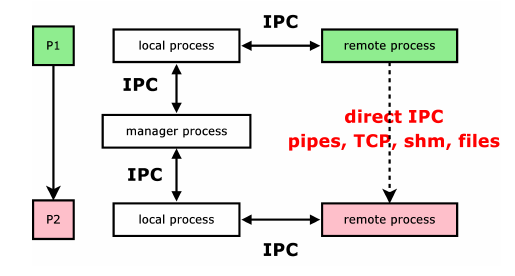
\includegraphics[width=1\textwidth]{figuras/ipc.png}
    \legend{Características dos mecanismos de comunicação \citeonline{sistemas-op-mazierro}}
    \label{fig:how-communication-works}
\end{figure}

\section{Cliente/Servidor}\label{sec:clientserver}

Também conhecido como arquitetura de duas camadas, o modelo cliente/service consiste em uma arquitetura em que a camada de apresentação se encontra no cliente e a camada de dados esta armazenada no servidor. Esta separação se opõe ao modelo centralizado amplamente utilizado.

O processamento dos dados é dividido em duas partes distintas. Uma parte é a requerente de dados (cliente), e a outra parte é a provedora dos dados (servidor). O cliente envia durante sua execução uma ou mais solicitações ao servidor para realizar alguma tarefa específica. É delea responsabilidade tanto de apresentar as informações para o usuário, quando executar as regras de negócio necessárias à aplicação. O servidor é responsável por armazenar os dados e prover um meio para que o cliente os consulte.

Desde a década de 1990, fornecedores de software desenvolvem e trazem ao mercado muitas ferramentas para simplificar o desenvolvimento de aplicativos para a arquitetura cliente/servidor de 2 camadas. Algumas das mais conhecidas são: Microsoft Visual Basic, Delphi da Borland e PowerBuilder da Sybase. Essas ferramentas combinadas com milhões de desenvolvedores que sabem usá-las, significa que a abordagem de duas camadas de cliente/servidor é uma solução econômica para certas classes de problemas.

Desde então, aplicações \textit{desktop} comunicando-se com o servidor de banco de dados era um caso de uso normal. A maior parte da lógica de negócios foi incorporada dentro da aplicação \textit{desktop}. Portanto, esse estilo de aplicativos cliente/servidor também foi chamado de \textit{fat clients}. 

\begin{figure}[ht]
    \centering
    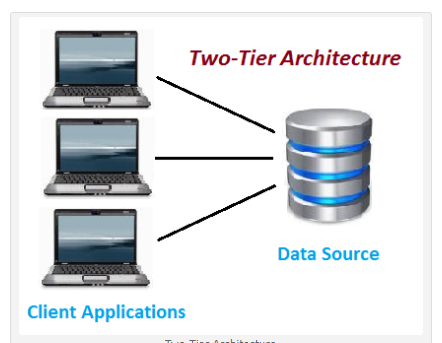
\includegraphics[width=0.8\textwidth]{figuras/two-tier.png}
    \caption{Comunicação em duas camadas}
    \label{fig:two-tier}
\end{figure}

A figura \ref{fig:two-tier} ilustra como a arquitetura em duas camadas funciona, mantendo uma comunicação direta entre cliente e servidor, sem intermediarios entre as duas pontas. Visto que neste modelo as regras de negocio estão presentes na camada de aplicação, ele é frequentemente aplicado em ambientes homogêneos. A camada de banco de dados e a camada de aplicação estão fisicamente próximos, o que oferece um bom desempenho para as aplicações.

Por outro lado, o modelo cliente servidor em duas cadamas tem grandes desafios de escabilidade. Quando multiplos usúarios executam requisições simultaneas, a aplicação perde muito desempenho, dado ao fato que cada cliente precisa de conecções separadas e memória de CPU para processar as requisições. Entretando, um dos maiores problemas na arquitetura em duas camadas ocorre quando há mudanças na estrutura do banco de dados. A maioria das aplicações usadas para interação depende da estrutura do banco de dados criando um problema quando é preciso remodela-lo, já que as aplicações são dependentes da estrutura predominante.

\section{Aplicações Monolíticas}\label{sec:monolitico}
Em engenharia de software, uma aplicação monolítica descreve uma única aplicação de software em camadas no qual a interface de usuário e código de acesso aos dados são combinados em um único programa a partir de uma única plataforma.

Uma aplicação monolítica é autônoma e independente de outras aplicações de computação. A filosofia do projeto consiste em um aplicativo que não é responsável apenas por uma determinada tarefa, mas que também pode executar todos os passos necessários para completar uma determinada função.

A arquitetura monolítica é um padrão comumente usado para o desenvolvimento de aplicações corporativas. Esse padrão funciona razoavelmente bem para pequenas aplicações, pois o desenvolvimento, testes e implantação de pequenas aplicações monolíticas é relativamente simples. No entanto, para aplicações grandes e complexas, a arquitetura monolítica torna-se um obstáculo ao desenvolvimento e implantação, dificulta a utilização de uma entrega contínua, além de limitar a adoção de novas tecnologias. Para grandes aplicações, faz mais sentido usar uma arquitetura de microservices, que divide a aplicação em um conjunto de serviços.

\section{SOA - Service Oriented Architecture}\label{sec:soa}

Este documento e seu código-fonte são exemplos de referência de uso da classe
\textsf{abntex2} e do pacote \textsf{abntex2cite}. O documento exemplifica a elaboração de trabalho acadêmico produzido conforme a ABNT NBR 14724:2011 \emph{Informação e documentação - Trabalhos acadêmicos - Apresentação}.

O modelo apresentado é baseado no ``Modelo Canônico'' criado pela equipe do projeto \abnTeX\, e implementa os requisitos das normas da ABNT. Uma lista completa das normas
observadas pelo \abnTeX\ é apresentada em \citeonline{abntex2classe}. Aqui, está apresentada a forma que o modelo será utilizado no curso de Bacharelado em Sistemas de Informação do IFC - Araquari.

Este documento deve ser utilizado como complemento dos manuais do \abnTeX\ 
\cite{abntex2classe,abntex2cite,abntex2cite-alf} e da classe \textsf{memoir}
\cite{memoir}. 

Na introdução o autor coloca o problema ou a indagação que o levou a escrever o texto. A introdução nos dá, então, uma idéia do assunto tratado. Além disso, nela o autor coloca também o ponto de vista ou o ângulo sob o qual ele vai abordar o assunto e, às vezes, o método, ou seja, o caminho que vai seguir (se vai apresentar casos para chegar a uma generalização, ou se vai partir de um princípio geral e deduzir suas consequências).

Também na introdução, o tema é apresentado e esclarecido aos leitores as indicações de leitura do trabalho. Deve-se utilizar o projeto do TCC para colocar na introdução o objetivo principal, os objetivos específicos, o problema e a hipótese.

A respeito de materiais e métodos, pode-se falar sobre a infra-estrutura necessária para o trabalho, incluindo servidores, estações, equipamentos de rede, \emph{softwares} com suas respectivas versões e tudo o mais que for necessário.

A introdução termina com a apresentação dos demais capítulos do trabalho. O capítulo 2 contém o referencial teórico deste trabalho. No capítulo 3 é apresentado o desenvolvimento, o cenário, os testes e a discussão dos resultados. Por fim, temos a conclusão, onde discutiremos os resultados, as dificuldades encontradas e faremos sugestões de trabalhos futuros.